\subsection{Zustand: Bouncing-off}

Wie wir bereits wissen wird sich der Schwarm von einem Hindernis oder einer Wand abstoßen, wenn alle
Roboter kollidiert sind. Das Vorgehen ist relativ simpel und kann der folgenden Abbildung entnommen werden.\\

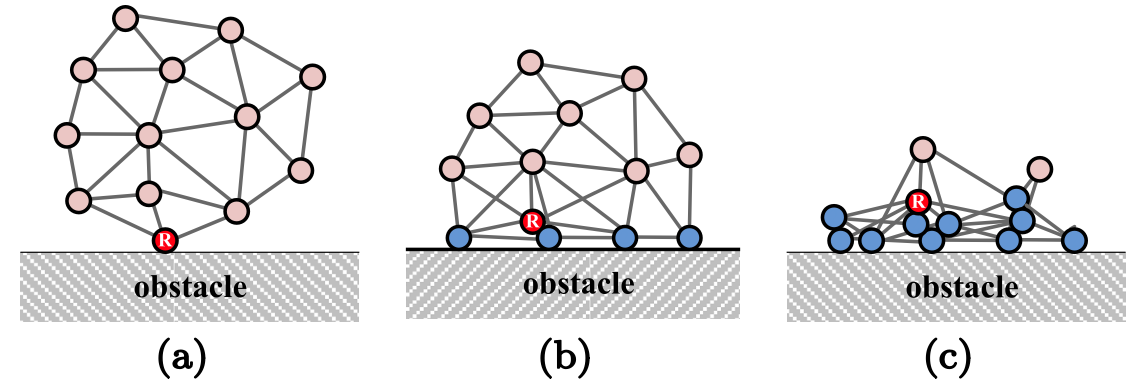
\includegraphics[width=3in]{images/Screenshot 2023-02-20 at 1.32.00 PM.png}
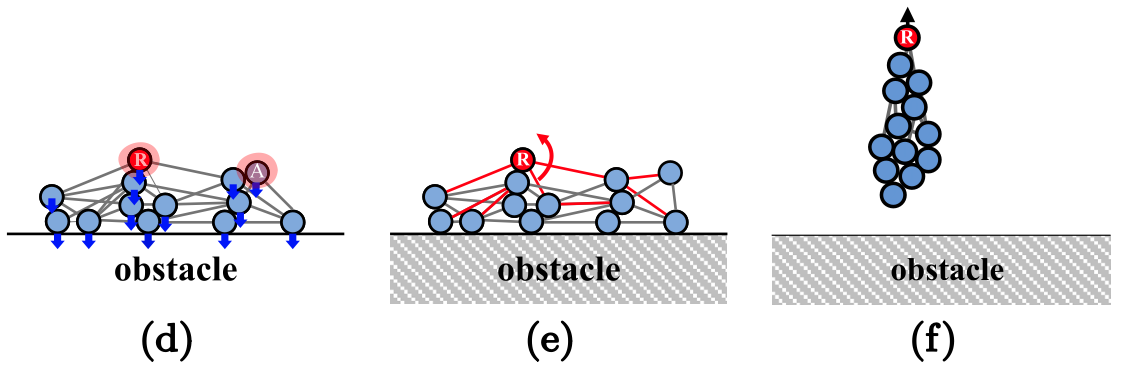
\includegraphics[width=3in]{images/Screenshot 2023-02-20 at 1.32.24 PM.png}

Von Schritt (a) zu Schritt (d) sehen wir, wie alle Roboter kollidieren, der Schwarm befindet sich ab dem
Zeitpunkt zwischen (d) und (e) also im Bouncing-off Zustand. Der Schwarm wählt nun ähnlich wie im Detouring
Zustand den Roboter aus, der am weitesten hinten im Schwarm ist. Das Kriterium, dass dieser Kandidat nicht
kollidiert sein darf entfällt logischerweise. Dieser neue Lead dreht sich nun vom Hindernis weg und die
anderen Roboter folgen wieder in einer Eltern-Kind-Beziehung. Wurde der maximale Baumwinkel wieder
unterschritten und ist kein Roboter mehr kollidiert, geht der Schwarm auch hier in den Reconstruction Zustand
über.